\documentclass{article}
\usepackage[utf8]{inputenc}
\usepackage{mathtools}
\usepackage{indentfirst}
\usepackage{verbatim}
\usepackage{gensymb}
\usepackage{graphicx}


\title{Math}
\author{Nathan Ueda}
\date{January 2024}

\begin{document}

\maketitle

\section{Stochastic Matrices}
\subsection{Stochastic Matrices}
    \begin{itemize}
        \item Informal definition: A square matrix that represent 
        transitions between different random states. Elements within a 
        stochastic matrix represent probabilities. This implies that each 
        element must be nonnegative and each row must sum to 1.
        \item Formal definition: A matrix $ \Phi \in R^{N \times N} $ is a 
        stochastic matrix if:
        \begin{itemize}
            \item all elements are positive: $ \Phi_{ij} \ge 0 \text{ for 
            all } i,j $
            \item each row sums to 1: $ \Sigma_j \Phi_{ij} = 1 \text{ for 
            all } i $
        \end{itemize}
    \end{itemize}

\subsubsection{Intepretations}
\begin{itemize}
    \item $P(s_{t+1} = n | s_t = m) = \Phi_{mn} $: This says that the element
    $ \Phi_{mn} $ represents the probability of the next state, $ s_{t+1} $ 
    being equal to $ n $ given that the current state, $ s_t $ is the $ m $th 
    state for all possible states $ s \in \{1, \dots, N\} $.
\end{itemize}

\subsubsection{Examples}
\begin{enumerate}
    \item 3-State Markov Process: Stochastic Matrix $ \Phi = \begin{bmatrix}
        0.8 & 0.2 & 0 \\
        0 & 0 & 1 \\
        0.05 & 0.95 & 0 
        \end{bmatrix} $
        \begin{center}
            \centering
            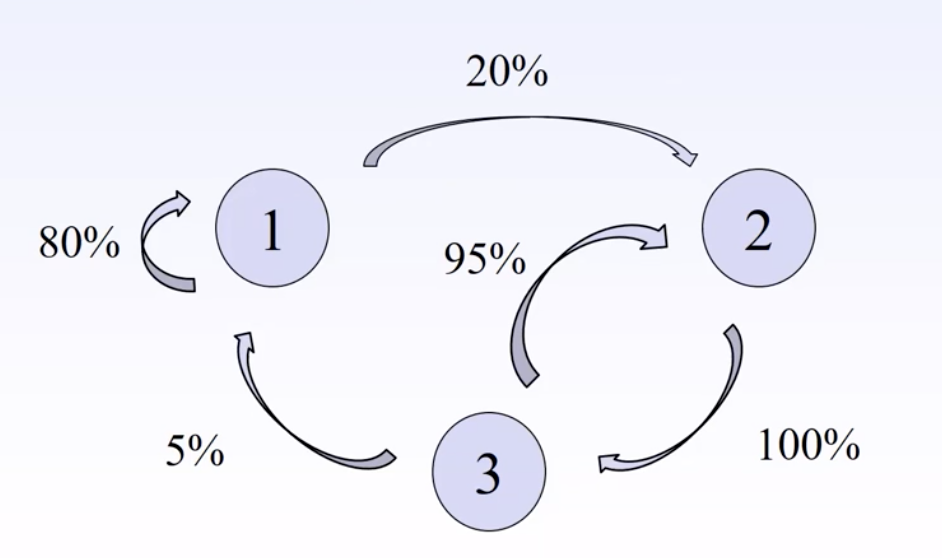
\includegraphics[width=0.8\textwidth]{imgs/stochastic_matrices1.png} \\
            \textit{Each node is a state. Each edge represents the probability of 
            transitioning from some state to another.}
        \end{center}
\end{enumerate}

\subsection{Discrete Kolmogorov Backward Equations}
\begin{itemize}
    \item Informal definition: 
    A formula to represent the expected value of some payoff function (i.e. for
    an option) depending upon what state we are in the future.
    \item Formal definition: For function $ F : \{ 1, \dots, N \}  \rightarrow R
    , $ define $ F(j) = f_j, f \in R^N $.
    \begin{itemize}
        \item $ F $ is the `payoff function' and $ f_j $ is the payoff, given we 
        are in state $ j $ at some future specified time.
    \end{itemize}
\end{itemize}

\subsubsection{Intepretations}
\begin{enumerate}
    \item $ \Phi^2 = \Phi \Phi $: The transition probabilities between two 
    periods, $ t $ and $ t + 2 $.
    \item $ \Phi^n $: The transition probabilities between n periods, $ t $ and
    $ t + n $.
    \item $ {[\Phi^{T-t}]}_{ij} = P(s_T = j | s_t = i) $: The probability of 
    being in state $ j $ after $ t $ periods, given that we are in state $ i $
    currently (at time $ t $) is the $ ij $-th element of the stochastic matrix
    $ \Phi^{T-t} $.
    \item $ E[F(s_T) | s_t = j] = {[\Phi^{T-t}f]}_j $: The expected payoff at 
    period $ T $, given that we are currently in state $ s_t = j $ at period 
    $ t $, is the $ j $-th element of the vector resulting from taking the 
    product of $ \Phi^{T-t} $ and the payoff function $ f $. 
    \begin{itemize}
        \item $ {[\Phi^{T-t}f]}_j = \Phi_{j1}^{T-t} f_1 + \cdots + \Phi_{jN}^{T-t} f_N $
    \end{itemize}
\end{enumerate}

\subsubsection{Examples}
\begin{enumerate}
    \item 3-State Markov Process: Stochastic Matrix $ \Phi = \begin{bmatrix}
        0.8 & 0.2 & 0 \\
        0 & 0 & 1 \\
        0.05 & 0.95 & 0 
        \end{bmatrix} $, \\
        $ \Phi^2 = \begin{bmatrix}
            0.64 & 0.16 & 0.2 \\
            0.05 & 0.95 & 0 \\
            0.04 & 0.01 & 0.95 
            \end{bmatrix} $
    \begin{center}
        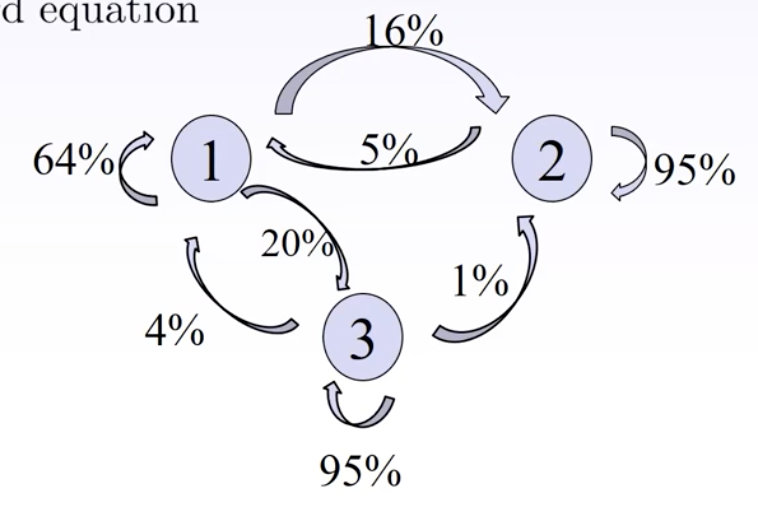
\includegraphics[width=0.8\textwidth]{imgs/stochastic_matrices2.png} \\
        \textit{Each node is a state. Each edge represents the probability of 
        ending up in the state at the end of the arrow, given we are in the 
        state at the tail of the arrow 2 periods prior.}
    \end{center}
\end{enumerate}

\subsection{Discrete Kolmogorov Forward Equations}
\begin{itemize}
    \item Informal definition: An equation useful in determining the distribution
    of us being in a specific state $ t $ periods into the future. 
    \item Formal definition: 
    \begin{itemize}
        \item Probability vector: a vector $ p \in R^N $ such that:
        \begin{itemize}
            \item $ p_i \ge 0 $
            \item $ \Sigma_i p_i = 1 $
        \end{itemize}
        \item Stationary distribution: a probability vector for a stochastic
        matrix, $ \Phi $, such that $ p = \Phi^* p $ (i.e. $ p $ is a left
        eigenvector of $ \Phi^* $ with an eigenvalue of 1) ($ \Phi^* $ is used 
        to denote the transpose).
        \item Discrete Kolmogorov Forward Equation: if the probability vector at
        $ t $ is $ p^t $, then at time $ T $, the probability vector for being
        in any given state is $ {(\Phi^*)}^{T-t}p^t $.
    \end{itemize}
    \item To ensure a stochastic matrix has a unique stationary distribution, 
    two criteria must be fulfilled:
    \begin{enumerate}
        \item The matrix must be \textbf{irreducible}. As stochastic matrix is said to be 
        irreducible if, for each $ i,j $, there exists $ k > 0 $ such that $ 
        {(\Phi^k)}_{ij} > 0$. In other words, there exists some path that has a 
        non-zero probability between any two states.
        \item The Markov chain is \textbf{aperiodic}. The \textbf{period} of 
        state $ i $, is $ k_i $, where $ k_i $ is the greatest common divisor of 
        the set $ \{n | {(\Phi^n)}_{ii} > 0\} $. If $ k_i = 1 $ for $ i = 1, 
        \dots, n $, then $ \Phi $ is aperiodic. In other words, to be aperiodic 
        means there is no cyclicality in the number of steps it takes to get 
        back to some starting state. 
    \item \textbf{Perron-Frobenius Theorem}: Consider an irreducible, aperiodic
    stochastic matrix $ \Phi $. Then $ \Phi $ has a unique stationary 
    distribution with strictly positive elements.
    \begin{itemize}
        \item All other left eigvenvalues of $ \Phi, \lambda_2, \dots, 
        \lambda_N, $ have $ |\lambda_i| < 1 $.
        \item All other left eigenvectors of $ \Phi $ have at least one 
        nonpositive element. 
    \end{itemize}
    \end{enumerate}
\end{itemize}
\subsubsection{Intepretations}
\begin{enumerate}
    \item $ \Phi^{1000} = \begin{bmatrix}
        0.111 & 0.444 & 0.444 \\
        0.111 & 0.444 & 0.444 \\
        0.111 & 0.444 & 0.444
        \end{bmatrix} $: This is the transition matrix 1000 periods into the 
        future. Each column has the same values. This means regardless of which
        state we start in, we have the same probability of ending up in any
        state 1000 periods later. This implies there is a limiting distribution 
        $ \textbf{p} = (0.111, 0.444, 0.444)' $ regardless of the initial state. 
        Note: there is not always a limiting distribution. 
\end{enumerate}

\end{document}
